% Material found at https://www.elsevier.com/authors/author-schemas/latex-instructions

\documentclass{elsarticle}

\usepackage{lineno,hyperref}
\modulolinenumbers[5]

%=== Added for MU paper ====
\usepackage{color,soul} %% this was needed to have highlighted text
\usepackage{graphicx}
\usepackage{hyperref}
\usepackage{amsmath}
\usepackage{mathtools}
\usepackage{nomencl}
\makenomenclature
\graphicspath{{./figures/}}

\journal{Reliability Engineering \& System Safety}

%%%%%%%%%%%%%%%%%%%%%%%
%% Elsevier bibliography styles
%%%%%%%%%%%%%%%%%%%%%%%
%% To change the style, put a % in front of the second line of the current style and
%% remove the % from the second line of the style you would like to use.
%%%%%%%%%%%%%%%%%%%%%%%

%% Numbered
\bibliographystyle{model1-num-names}

%% Numbered without titles
%\bibliographystyle{model1a-num-names}

%% Harvard
%\bibliographystyle{model2-names.bst}\biboptions{authoryear}

%% Vancouver numbered
%\usepackage{numcompress}\bibliographystyle{model3-num-names}

%% Vancouver name/year
%\usepackage{numcompress}\bibliographystyle{model4-names}\biboptions{authoryear}

%% APA style
%\bibliographystyle{model5-names}\biboptions{authoryear}

%% AMA style
%\usepackage{numcompress}\bibliographystyle{model6-num-names}

%% `Elsevier LaTeX' style
%\bibliographystyle{elsarticle-num}
%%%%%%%%%%%%%%%%%%%%%%%

\begin{document}

\begin{frontmatter}

\title{Assembling Multiple Models within the RAVEN framework: From High-Fidelity Tools to Surrogate Models}
%% \tnotetext[mytitlenote]{Fully documented templates are available in the elsarticle package on \href{http://www.ctan.org/tex-archive/macros/latex/contrib/elsarticle}{CTAN}.}

%% Group authors per affiliation:
\author{Andrea Alfonsi}
\address{andrea.alfonsi@inl.gov}

\author{Diego Mandelli}
\address{diego.mandelli@inl.gov}

\author{Cristian Rabiti}
\address{cristian.rabiti@inl.gov}

\author{Carlo Parisi}
\address{carlo.parisi@inl.gov}

\begin{abstract}
  Risk importance measures are indexes that are used to rank systems, 
structures and components (SSCs) using risk-informed methods. 
The most used/known measures are: Risk Reduction Worth (RRW), 
Risk Achievement Worth (RAW), Birnbaum (B) and Fussell-Vesely (FV). 
Once obtained from classical Probabilistic Risk Analysis (PRA) analyses, 
these risk measures can be effectively employed to relatively rank
component importance.
In contrast to classical PRA methods, 
Dynamic PRA methods couple stochastic models with safety analysis 
codes to determine risk associate to complex systems such as nuclear 
plants. Compared to classical PRA methods, simulation-based approaches
can evaluate with 
higher resolution the safety impact of timing and sequencing of events 
on the accident progression. 
The objective of this paper is to present a series of methods that 
can be employed to measure risk importance of components which are 
part of complex systems such as nuclear power plants.
The first set of measures are directly derived from classical risk 
importance measures (e.g., RRW, RAW, B and FV) and that can be employed
to any Dynamic PRA analysis.
In addition, we provide a set of risk importance measures that capture the 
dynamic nature of the problem and provide insight related to plant safety 
margins.

\end{abstract}

\begin{keyword}
%% keywords here, in the form: keyword \sep keyword
RAVEN \sep Uncertainty Quantification \sep Probabilistic Risk Assessment \sep Surrogate Models 
\end{keyword}

\end{frontmatter}

\linenumbers

\printnomenclature[1in]

\nomenclature{LWRS}{Light Water Reactor Sustainability}
\nomenclature{PWR}{Pressurized Water Reactor}
\nomenclature{RAVEN}{Risk Analysis Virtual ENvironment}
\nomenclature{ROM}{Reduced Order Model}
\nomenclature{SFP}{Spent Fuel Pool}
\nomenclature{ROM}{Reduced Order Modeling}
\nomenclature{RISMC}{Risk Informed Safety Margin Characterization}	

\section{Introduction}
\label{sec:introduction}
RAVEN (\textbf{R}isk \textbf{A}nalysis \textbf{V}irtual \textbf{EN}vironment)~\cite{Nureg1150}  is one of the many INL-developed software tools researchers can 
use to identify and 
increase the safety margin in complex systems (e.g. Nuclear Power Plants). It is a modular or ``plug-able'' framework that can be coupled with other computer 
modeling systems. RAVEN is capable to agnostically communicate with any system 
code. This agnosticism includes providing Application Programming Interfaces (APIs). These APIs are used to allow RAVEN to interact with any code as long as all 
the parameters that need to be perturbed are accessible through input files or via python interfaces. 
As a generic software framework, RAVEN is designed to perform parametric and probabilistic analysis based on the response of complex system codes. RAVEN is 
capable of investigating the system response as well as the input space using standard sampling techniques (e.g Monte Carlo, Grid, or Latin Hyper Cube), but its 
strength is focused toward system feature discovery, such as limit surfaces (i.e. separating regions of the input space leading to system failure, using dynamic 
supervised learning techniques), and advanced data analysis methodologies (i.e. Topology-based domain decomposition, Data Mining, Clustering, etc.).

The development of RAVEN has begun in 2012 to satisfy the need to provide a modern risk evaluation framework. RAVEN principal assignment is to provide the 
necessary software and algorithms in order to employ the concept developed by the Risk Informed Safety Margin Characterization (RISMC) path-
way~\cite{RISMC}. 
RISMC is one of the pathways defined within the Light Water Reactor Sustainability (LWRS) program. In the RISMC approach, the goal is not just specifically 
identifying the frequency of an event potentially leading to a system failure, but also to analyze the ``distance'' and the drivers toward the happening of key 
safety-related events. This approach may be used in identifying and increasing the safety margins related to those events. A safety margin is a numerical value 
quantifying the probability that a safety metric (e.g. as peak pressure in a pipe) is exceeded under certain conditions. The initial development of RAVEN has 
been focused on providing dynamic risk assessment capability to RELAP-7~\cite{RELAP7}, currently under development at the INL. All the methodologies
developed have been modularized in order to be applied to any computer modeling system (e.g., BISON, RELAP-7, RELAP5-3D, MELCOR, etc.).

The aim of this manuscript is to present a peculiar capability within the RAVEN framework named \textit{``EnsembleModels''}.

RAVEN is currently able to construct multi-targets Reduced Order Models (Ref.4), which are aimed to represent the response of a system (in a 
fixed configuration) for multiple Figures of Merits (FOMs) and time-dependent ROMs (see Ref.5). These capabilities represent the initial steps for a larger 
implementation about the interaction of multiple models. In fact, in several cases, multiple models need to interface with each other since the initial conditions of 
one are dependent on the outcomes of another.
To better understand the problem that here is solved, it is useful to consider two simple examples:
\begin{enumerate}
  \item The following problem is considered: a weather forecast simulation code ``a'' is used to compute the external (i.e. ambient) temperature in a certain location. 
  A second model ``b'' is inquired to compute the average temperature in a room having as boundary condition, among several others, the external ambient 
  temperature. The response of the model ``b'' depends on the outcome of the model ``a'';
   \item Two different simulation codes are considered: a) a code that is meant to compute the thermal conductivity of the ceramic Uranium Dioxide (UO2) as 
   function of the Temperature, and b) a Thermal-hydraulic (TH) code that is used to compute the Temperature field of a reactor, whose heat conduction depends on 
   the thermal conductivity value. As easily inferable, the two models are mutual dependent, determining in a non-linear system of equations.
\end{enumerate}
The two reported examples are only aimed to illustrate the reason why the creation of a framework to make interact different models is a key development for the 
advancement of RAVEN as a comprehensive calculation flow driver. Before reporting how the ensemble-models have been implemented, it is necessary to briefly 
describe the representative Model ``entities'' that are available in RAVEN.



\begin{figure}
    \centering
    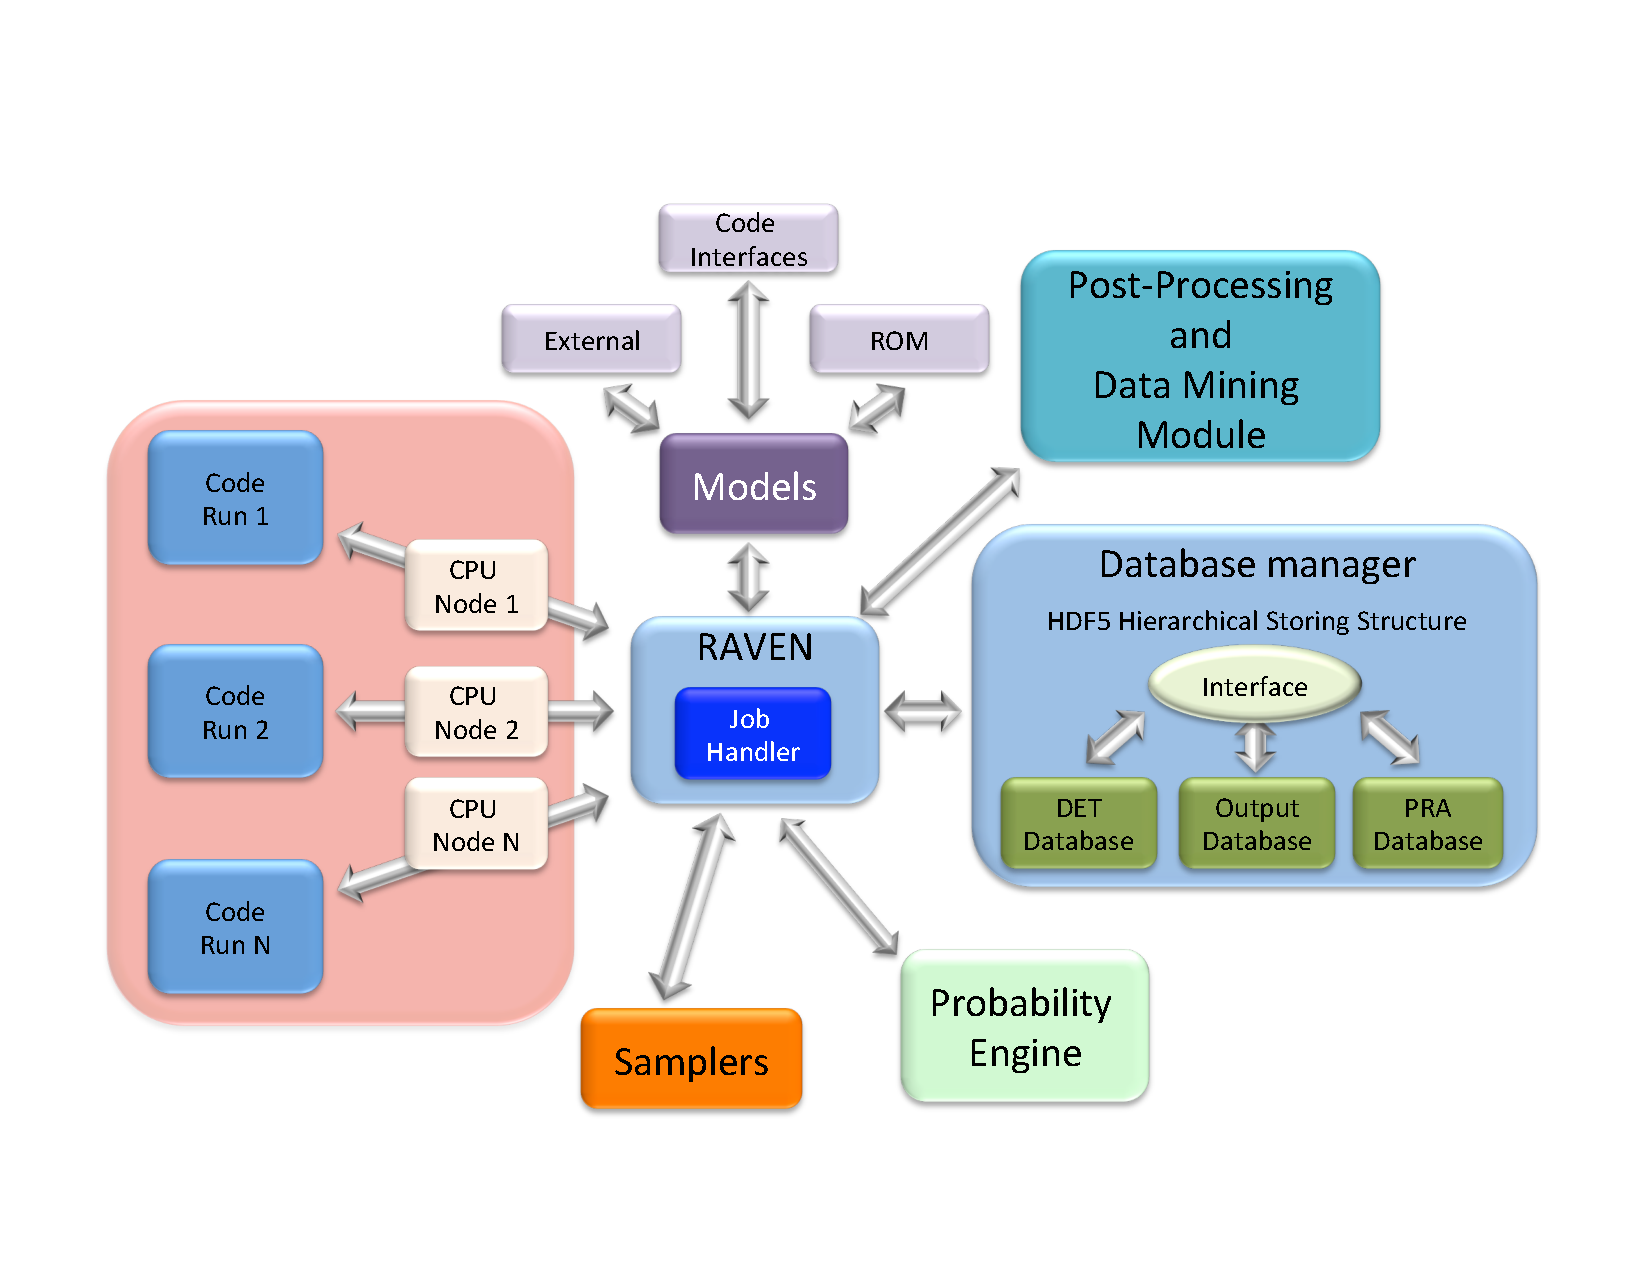
\includegraphics[scale=0.5]{raven.pdf}
    \caption{RAVEN}
    \label{fig:raven}
\end{figure}

\section{Model Entities in RAVEN}
\label{sec:models}
As already metioned, 
the Model entity, in the RAVEN environment, represents a ``connection pipeline'' 
between the input and the output space. The RAVEN framework does not own any 
physical model (i.e. it does not posses the equations needed to simulate/model 
systems or phenomena), but implements APIs by which any generic model can be 
integrated and 
interrogated. In the RAVEN framework four different model categories (entities) are 
defined:
\begin{itemize}
   \item \textit{Codes};
   \item \textit{Externals};
   \item \textit{ROMs};
   \item \textit{PostProcessors}.
\end{itemize}

The \textit{Code} model represents the interface object that establishes the communication pipe between RAVEN and any driven code. Currently, RAVEN has APIs for 
several different codes:
\begin{enumerate}
  \item RELAP5-3D, the most widely used Safety Code (thermal-hydraulic);
  \item RELAP-7, safety code eventual future replacement of RELAP5-3D code;
  \item any MOOSE-based application;
  \item SAS4A/SASSYS-1, safety analysis code for fast reactors (Argonne)
  \item Modelica, object-oriented, declarative, multi-domain modeling language for component-oriented modeling of complex systems;
  \item MELCOR, engineering-level computer code that models the progression of severe accidents in light-water reactor nuclear power plants (contributed by the 
           University of Rome “La Sapienza”);
  \item MAAP5, computer code that models the progression of severe accidents in light-water reactor nuclear power plants (coupling performed by the Ohio State 
          University).         
\end{enumerate}

The data exchange between RAVEN and the driven code can be performed either by direct software interface or by files.
The
If the system code is parallelized, the data exchanging by files is generally the way to 
follow since it can be much more optimized in large clusters.

The External model allows the user to create, in a Python file (imported, at run-time, in 
the RAVEN framework), its own model (e.g. set of equations representing a 
physical model, connection to another code, control logic, etc.). This model will be 
interpreted/used by the framework and, at run-time, will become part of RAVEN 
itself.
\begin{figure}
    \centering
    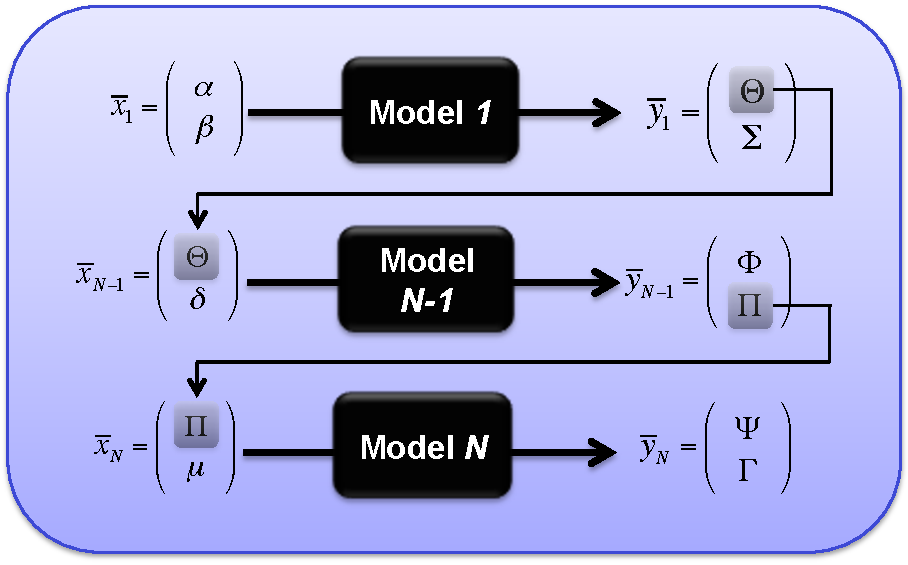
\includegraphics[scale=0.6]{EnsembleModelChain.pdf}
    \caption{Example of an \textit{EnsembleModel} constituted by 3 sequential sub-models}
    \label{fig:ensembleModelChain}
\end{figure}
The ROM (Reduced Order Model) represents an API to several different algorithms. A 
ROM is a mathematical representation of a system, used to predict a selected 
output space of a physical system. The creation and sub-sequential usage of a ROM 
involves a procedure named ``training''. The ``training'' is a process that uses 
sampling of the physical model to improve the prediction capability (capability to predict 
the status of the system given a realization of the input space) of the ROM. 
More specifically, in RAVEN the ROM is trained to emulate a high fidelity numerical 
representation (system codes) of the physical system.
The Post-Processor model is aimed to manipulate the data generated, for example, 
employing a sampling strategy. In RAVEN several different post-processors are 
available: 1) Statistics Post-Processor, aimed to compute all the statistical figure of 
merits (e.g. expected values, variance, skewness, covariance matrix, sensitivity 
coefficients, etc.); 2) Limit Surface, which computes the Limit Surface, inquiring a goal 
function (i.e. a function that determines if a certain coordinate in the input space 
led to a failure or success), and so many others.
As already mentioned, in several cases multiple models need to interface with each 
other since the initial conditions of some are dependent on the outcomes of others. 
In order to face this problematic in the RAVEN framework, a new model category (e.g. 
class), named EnsambleModel, has been implemented. This class is able to 
assemble multiple models of other categories (i.e. Code, External Model, ROM), 
identifying the input/output connections, and, consequentially the order of execution 
and which sub-models can be executed in parallel.

\section{EnsembleModel in RAVEN}
\label{sec:ensembleModel}
Before analyzing in detail how the \textit{EnsembleModel}  capability has been 
developed in the
RAVEN framework, it is worth to report a couple of schematic cases that show how the 
input/output interconnections
determine the order of execution of the sub-models. Figure ~\ref{fig:ensembleModelChain} reports an example of an \textit{EnsembleModel} that is 
constituted by 3
sub-models (ROMs, Codes, or External Models). As it can be noticed:
\begin{itemize}
  \item The Model 2 is connected with the Model 1 through the variable (Model 1 output 
  and Model 2 input);
  \item The Model 3 is connected with the Model 2 through the variable (Model 2 output 
  and Model 3 input);
\end{itemize}
In this case, the \textit{EnsembleModel} is going to drive the execution of all the sub-
models in a serial sequence, since each model (except the Model 1) is dependent on 
one of the outcomes of previously executed.

\begin{figure}
    \centering
    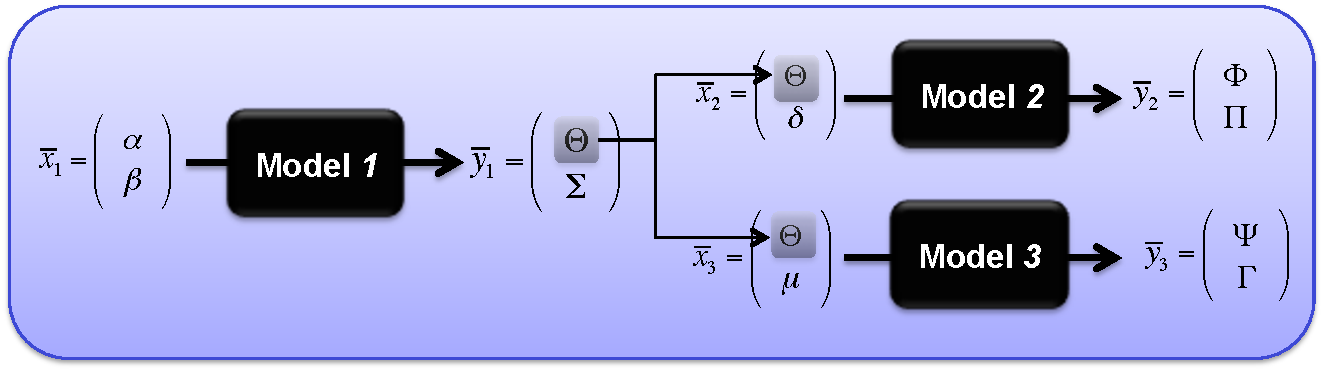
\includegraphics[scale=0.6]{EnsembleModelChainParallel.pdf}
    \caption{Example of a  \textit{EnsembleModel} constituted by 3 sub-models, 2 of which can be run independently}
    \label{fig:ensembleModelChainParallel}
\end{figure}

In Figure ~\ref{fig:ensembleModelChainParallel} another example is reported. In this 
case, the Model 2 and Model 3 depend on the Model 1 only through an
output variable and they are not linked to each other. For this reason, the 
\textit{EnsembleModel} executes the Model 2 and Model 3 in parallel, after inquiring the 
Model 1.

In several cases, the input of a model depends on the output of another model whose 
input is the output of
the initial model. In this situation, the system of equation is non-linear and an iterative 
solution procedure needs
to be employed. The \textit{EnsembleModel} entity in RAVEN is able to detect the non-
linearity of the sub-models’
assembling and activate the non-linear solver: Picard’s iterative scheme. 
\begin{figure}
    \centering
    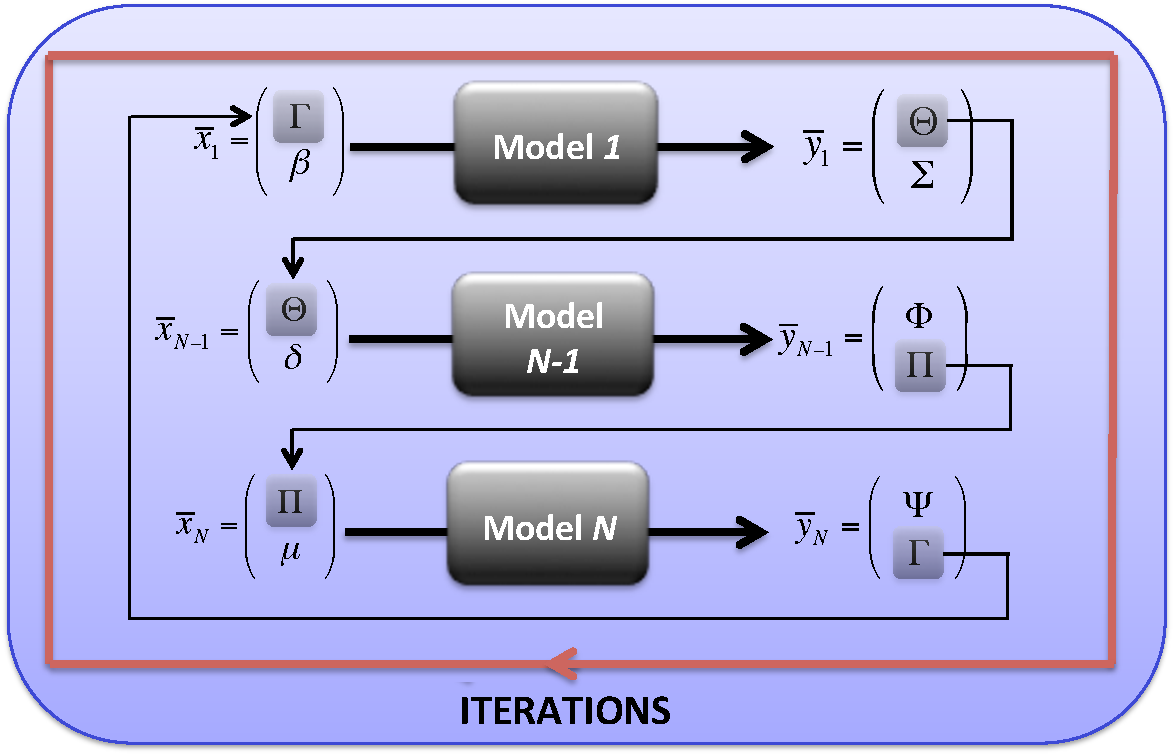
\includegraphics[scale=0.6]{EnsembleModelIterations.pdf}
    \caption{\textit{EnsembleModel} resolving in a non-linear system of equations – Iterative scheme}
    \label{fig:ensembleModelPicard}
\end{figure}
Figure ~\ref{fig:ensembleModelPicard} shows an example of when the
\textit{EnsembleModel} entity activates the Picard’s iteration scheme, which ends when 
the residue norm (between an iteration and the other) falls below a certain input-
defined tolerance.

\begin{figure}
    \centering
    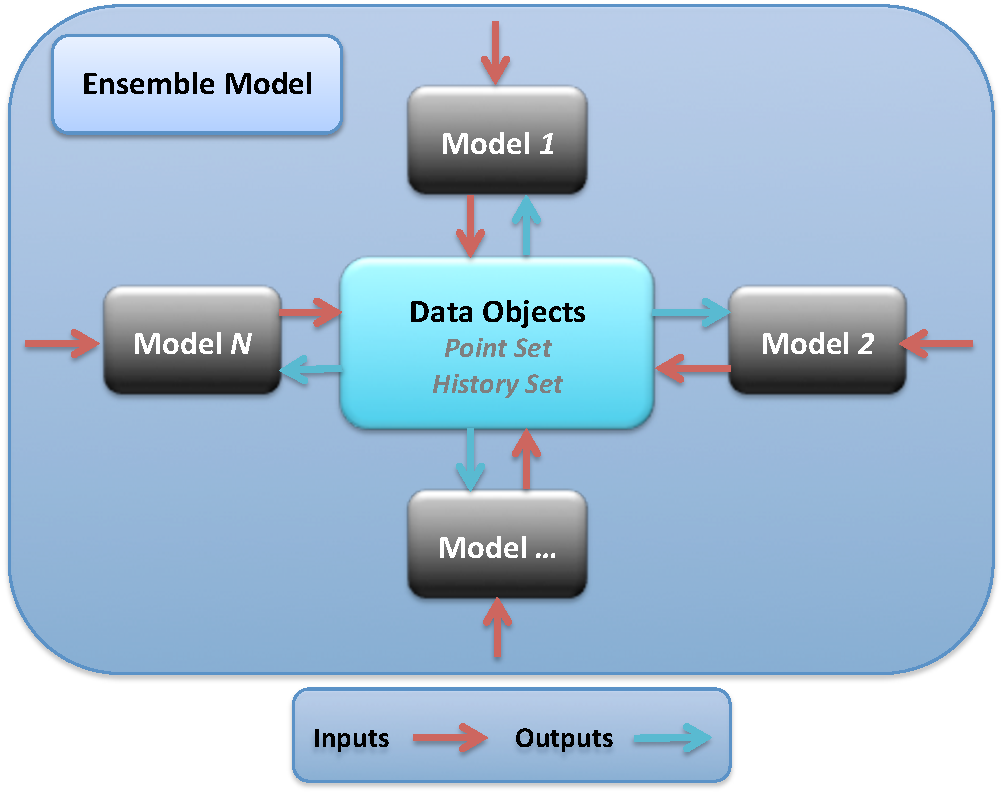
\includegraphics[scale=0.6]{EnsembleModelComunication.pdf}
    \caption{\textit{EnsembleModel} data exchange among sub-models}
    \label{fig:ensembleModelComunication}
\end{figure}

In RAVEN all the models’ outputs (e.g. whatever code output, etc.) are collected in an 
internal containers
(named DataObjects) that are aimed to store time-series and input/output data relations 
in a standardized
fashion; in this way, the communication of the output information among different 
entities (i.e. Models) can be
completely agnostic with respect to the particular type of output generated by a model. 
The Ensemble-Model
entity fully leverages this peculiarity in order to transfer the data from a Model to the 
other(s). 
Based on the Input/Output relations of each sub-models, the Ensemble-Model entity 
constructs the order of
their execution and, consequentially, the links among the different entities. 

%%%%%%%%%%%%%%
%    1-D figure of merits    %
%%%%%%%%%%%%%%
\subsection{EnsembleModel data infrastructure}
\label{subsec:ensemblemodelDataInfrastructure}
As already mentioned, the \textit{EnsembleModel} capability is primary aimed
to link different models in order to perform of combined analysis of different, for example,
physics. 
The initial infrastructure of the \textit{EnsembleModel}  was able to 
transfer information
among different models just in case of scalar quantities (e.g. peak clad temperature, 
constant thermal
conductivity, etc.). This limitation was connected to the fact that in RAVEN the 
concept of ``input realization''
was limited to scalar uncertainties (i.e. the RAVEN code was able to perturb the input 
space in terms of scalar
quantities). Since the increasing interest in using RAVEN also oriented to 
interconnection among heterogeneous
Models’ entities, the concept of treatable ``input realizations'' has been revised, including 
the possibility to process 1-D realizations. This addition determined the possibility to transfer
array-like FOMs among different models. 

Figure ~\ref{fig:ensembleModelComunication} schematically shows the communication 
piping established by the 
\textit{EnsembleModel} entity. It can be noticed how the sub-models share information (inputs/outputs data) using 
the \textit{DataObjects} entity as communication network.

\section{Application examples}
\label{sec:applications}
The \textit{EnsembleModel} capability 

In order to test the newly developed capability to process 1-D FOMs in an EnsembleModel configuration,
two models have been considered:
A pump controller model (Model B) for a hypothetical simplified PWR model (see Figure 4) has
been used. It consists of the following components:
o Reactor core (RX)
o Motor operated pump
o Pump digital controller
Data Objects
Point Set
History Set
Model 1
Model N Model 2
Model …
Inputs Outputs
Ensemble Model
8
o Heat exchanger (HX)
This system is responsible to remove the decay heat generated from the core (RX) in order to
avoid damage of the core itself. While we assumed that both the HS and the pump are perfectly
reliable components (i.e., no failure can be introduced), using [Ref] as a references, the digital
pump controller reliability model has been performed using a continuous time Markov Chain
formulation.



\begin{itemize}
   \item \textit{Codes};
   \item \textit{Externals};
   \item \textit{ROMs};
   \item \textit{PostProcessors}.
\end{itemize}


\begin{figure}
    \centering
    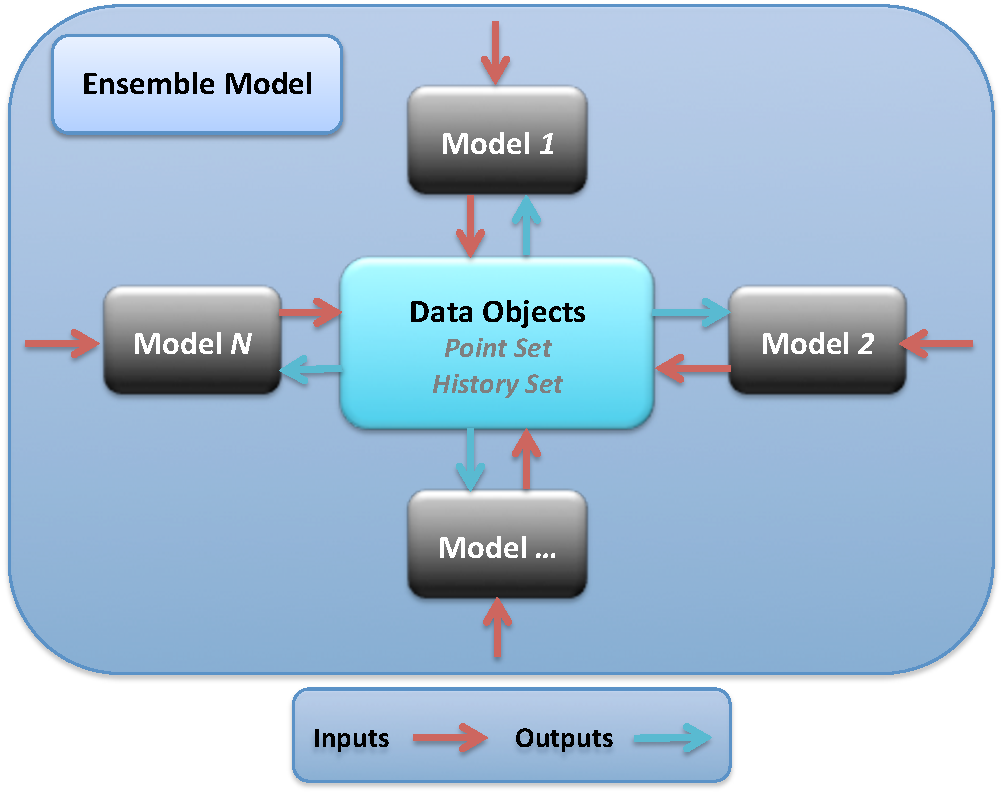
\includegraphics[scale=0.6]{EnsembleModelComunication.pdf}
    \caption{\textit{EnsembleModel} data exchange among sub-models}
    \label{fig:ensembleModelComunication}
\end{figure}


\section{Conclusions}
\label{sec:conclusions}
In this paper, a newly developed capability of the RAVEN code has been shown. Through the Ensemble-Model entity, RAVEN is able to combine multiple models (i.e. Simulation Codes, Reduced Order Models, etc.), constructing a pipe network in order to transfer information among them. The addition of the Picard’s iteration scheme lets the user solving combinations of models that resolve in non-linear systems. 
The paper shows the early results for implementation of an ensemble approach for the coupling of surrogate models representing a multi-physics problem. While this is an initial implementation, the developed structure seems to support current needs and will be eventually extended in the future in order to couple codes whose input/output space is represented by high-density fields (e.g. temperature profiles in each nodal kinetic zones, etc.). This capability builds a complex system representation, even when the original models were not coupled, but just coupled their surrogate. Two applications are relevant for reliability analysis: (1) the possibility to build surrogate representation of a complex system, starting from libraries of surrogate models for each component, and (2) software implementation present during the first stage of surrogate model coupling when responses are high-density fields. 
The Ensemble-Model capability in RAVEN is currently used to couple a fuel performance code (Bison) and the T-H system code RELAP5 in order to analyze LOCA scenarios.ion.


\section*{References}

\bibliography{main}

\end{document}